\chapter{Classification and Decision Thresholds}
\label{chap:classification}
\chapterguide
  {You should understand train/test evaluation and numeric prediction metrics.}
  {fit a binary logistic model, convert probabilities to decisions, construct a confusion matrix, and explain accuracy, precision, sensitivity, and specificity.}

\section{Classification predicts categories}
A binary classifier estimates evidence for one of two outcomes, such as fraud/not fraud, churn/stay, or malignant/benign. Many classifiers first produce a probability-like score and then apply a threshold to make a class decision.

For logistic regression,
\[
P(Y=1\mid x)=\frac{1}{1+e^{-\eta}},
\qquad
\eta=\beta_0+\beta_1x_1+\cdots+\beta_px_p.
\]


\section{Logistic regression models log-odds linearly}
The logistic curve converts the unconstrained linear predictor $\eta$ into a value between zero and one. Equivalently,
\[
\log\left(\frac{p}{1-p}\right)=\beta_0+\beta_1x_1+\cdots+\beta_px_p,
\]
so each coefficient changes the \term{log-odds} of the positive class conditionally on the other included variables. Exponentiating a coefficient gives an odds ratio for a one-unit feature change, but this remains an associational model unless the design supports causal interpretation.

\begin{utpfig}[Logistic transformation]{The S-shaped logistic function compresses extreme linear scores toward probabilities near 0 and 1 while mapping a score of zero to probability 0.5.}{fig:classification-sigmoid}
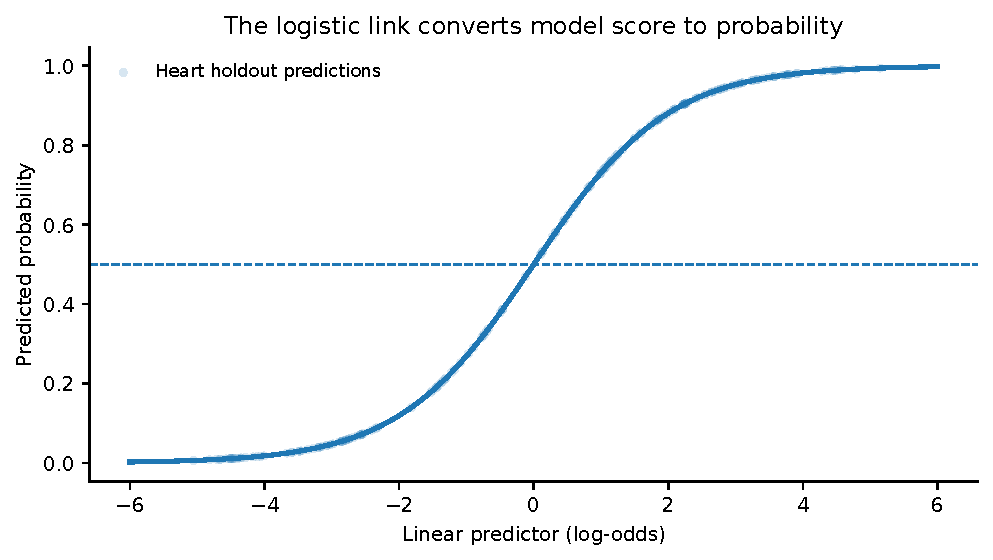
\includegraphics[width=0.80\linewidth]{figures_generated/classification_sigmoid.pdf}
\end{utpfig}

\section{The confusion matrix is the evaluation foundation}
\begin{dstable}
\begin{tabularx}{\linewidth}{@{}D{2.8cm}YD{5.5cm}@{}}
\toprule
\rowcolor{DSPaleBlue!92}
\textbf{Outcome} & \textbf{Meaning} & \textbf{Example in a medical screening context} \\
\midrule
True positive & predicted positive, actually positive & malignant case flagged \\
False positive & predicted positive, actually negative & benign case flagged \\
True negative & predicted negative, actually negative & benign case not flagged \\
False negative & predicted negative, actually positive & malignant case missed \\
\bottomrule
\end{tabularx}
\end{dstable}

From these counts:
\[
\text{Sensitivity}=\frac{TP}{TP+FN},\qquad
\text{Specificity}=\frac{TN}{TN+FP},\qquad
\text{Precision}=\frac{TP}{TP+FP}.
\]
Accuracy is \((TP+TN)/N\).


\begin{utpfig}[Confusion matrix from a held-out teaching split]{Counts retain the direction of each mistake. Reporting only accuracy would hide whether errors are mostly false positives or false negatives.}{fig:classification-cm}
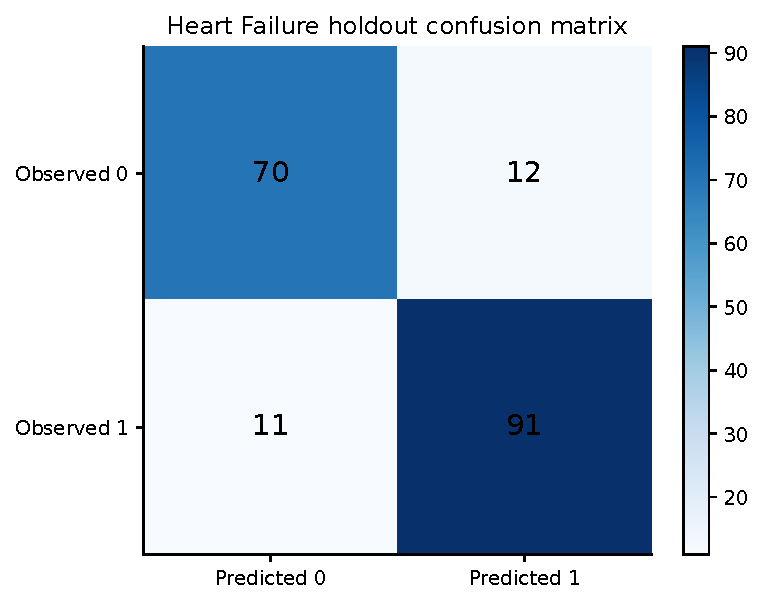
\includegraphics[width=0.58\linewidth]{figures_generated/classification_confusion_matrix.pdf}
\end{utpfig}

\section{Metrics answer different operational questions}
Sensitivity asks, ``Of the actual positives, how many did we find?'' Specificity asks the corresponding question for negatives. Precision asks, ``Of the cases we flagged positive, how many were actually positive?'' These denominators differ, so the metrics answer different questions.

Precision is especially sensitive to prevalence. A classifier can have similar sensitivity and specificity in two populations but very different precision if the event is much rarer in one population.


\section{Accuracy can fail on imbalanced data}
If 99\% of cases are negative, predicting ``negative'' every time yields 99\% accuracy and zero ability to find positives. Metric choice must reflect the operational cost of mistakes.

\begin{pitfall}
There is no universally correct threshold of 0.5. Lowering the threshold usually catches more positives but also creates more false positives. The right trade-off depends on consequences, prevalence, and downstream capacity.
\end{pitfall}


\begin{utpfig}[Where classification errors come from]{Predicted-score distributions for the two classes overlap. Moving the threshold changes which part of the overlap becomes false positive or false negative.}{fig:classification-overlap}
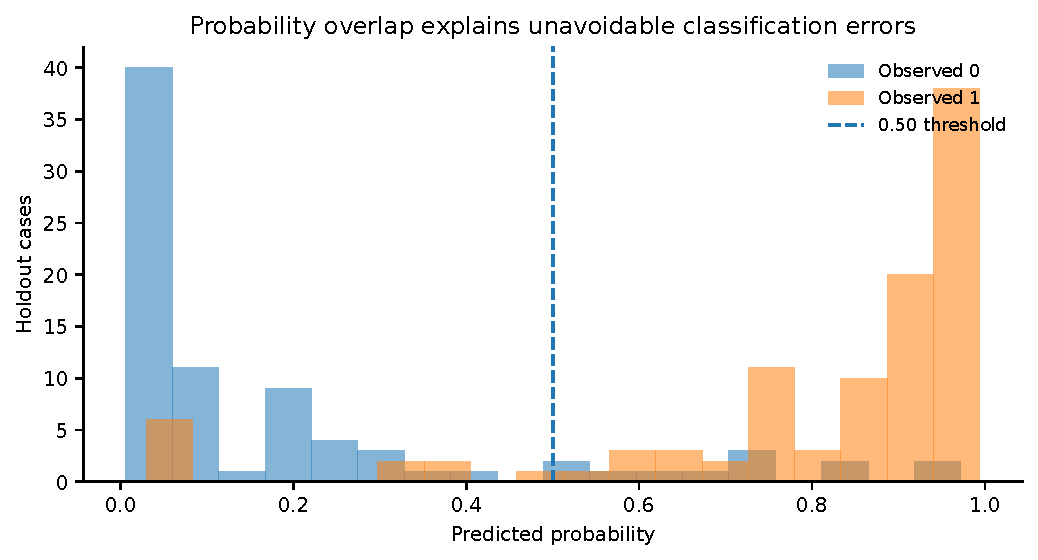
\includegraphics[width=0.82\linewidth]{figures_generated/classification_score_overlap.pdf}
\end{utpfig}


\begin{utpfig}[Threshold trade-off]{The probability model and the decision rule are separate. Changing the threshold can change false-negative and false-positive rates without refitting the model.}{fig:threshold-tradeoff}
\begin{tikzpicture}[x=\linewidth,y=1cm,
  stage/.style={draw=UTPBlue!65,fill=UTPPaleBlue,rounded corners=1.8mm,
    line width=0.7pt,text width=0.14\linewidth,
    minimum width=0.19\linewidth,minimum height=1.70cm,
    inner xsep=3mm,inner ysep=2.5mm,align=center,
    font=\scriptsize\color{UTPNavy}},
  flow/.style={-{Stealth[length=2.2mm,width=1.6mm]},
    line width=0.9pt,draw=UTPTeal}]
\node[stage,draw=UTPTeal!80,fill=UTPPaleTeal] (p) at (0.11,0)
  {\textcolor{UTPTeal}{\textbf{01  SCORE}}\\[5pt]
   \textbf{Model outputs}\\[4pt]
   Scores or probabilities};
\node[stage,draw=UTPOrange!80,fill=UTPPaleOrange] (t) at (0.37,0)
  {\textcolor{UTPOrange!85!black}{\textbf{02  THRESHOLD}}\\[5pt]
   \textbf{Choose cutoff}\\[4pt]
   Set the decision rule};
\node[stage] (d) at (0.63,0)
  {\textcolor{UTPBlue}{\textbf{03  DECIDE}}\\[5pt]
   \textbf{Class decisions}\\[4pt]
   Positive or negative};
\node[stage,draw=UTPTeal!80,fill=UTPPaleTeal] (c) at (0.89,0)
  {\textcolor{UTPTeal}{\textbf{04  EVALUATE}}\\[5pt]
   \textbf{Measure errors}\\[4pt]
   Confusion matrix and costs};
\draw[flow] (p.east) -- (t.west);
\draw[flow] (t.east) -- (d.west);
\draw[flow] (d.east) -- (c.west);
\end{tikzpicture}
\end{utpfig}


\begin{utpfig}[Metrics change with the threshold]{Sensitivity, specificity, and precision move differently as the same fitted model is evaluated at different decision thresholds. The choice must be connected to real error costs.}{fig:classification-threshold-metrics}
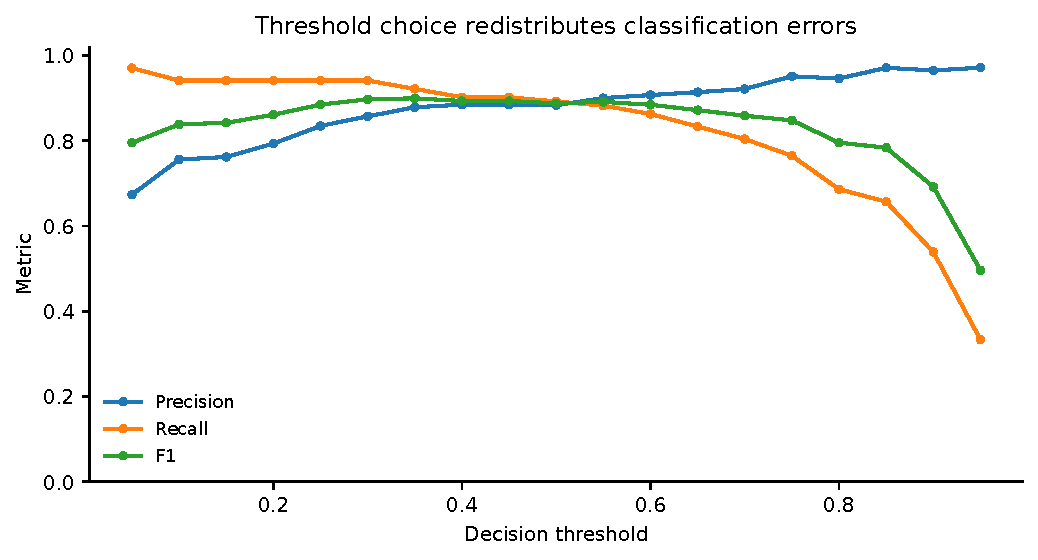
\includegraphics[width=0.84\linewidth]{figures_generated/classification_threshold_metrics.pdf}
\end{utpfig}

\section{Ranking, discrimination, and calibration are different}
A model can rank positive cases above negative cases well but still produce poorly calibrated probabilities. Conversely, a model can be reasonably calibrated overall yet weak at separating individual cases. Receiver-operating-characteristic and precision--recall curves summarise threshold behaviour across many cutoffs, while calibration plots compare predicted probabilities with observed event frequencies.

No single curve removes the need to choose an operating point when the system must ultimately make decisions.


\section{Probabilities need interpretation, not just labels}
A probability output lets analysts rank cases and choose thresholds. It should still be checked for calibration: among cases assigned around 0.8 risk, does the event occur roughly 80\% of the time? Calibration is distinct from classification accuracy.

\begin{workedexample}
In Lab 8 the target is \texttt{HeartDisease} in the bundled heart-failure dataset. The exercise demonstrates probability estimation and error metrics. It is not a clinical diagnostic system and should not be interpreted as one.
\end{workedexample}

\begin{keyidea}
Classification performance is multi-dimensional. Always ask which error matters, for whom, and under what prevalence and deployment conditions.
\end{keyidea}

\begin{quickcheck}
\begin{enumerate}
  \item Why can accuracy be misleading with rare positive cases?
  \item What does sensitivity measure?
  \item What happens to false positives and false negatives when a threshold changes?
  \item Why is calibration different from accuracy?
\end{enumerate}
\end{quickcheck}

\section{Two classification datasets, two different lessons}

The Heart Failure and Breast Cancer datasets both have binary outcomes, but they illustrate different modelling issues.

\begin{utpfig}[Heart-disease classes overlap in ordinary measurements]{Age and maximum heart rate provide useful signal but no clean separating boundary. Logistic regression therefore estimates a probability rather than claiming that one measurement combination deterministically defines disease.}{fig:class-heart}
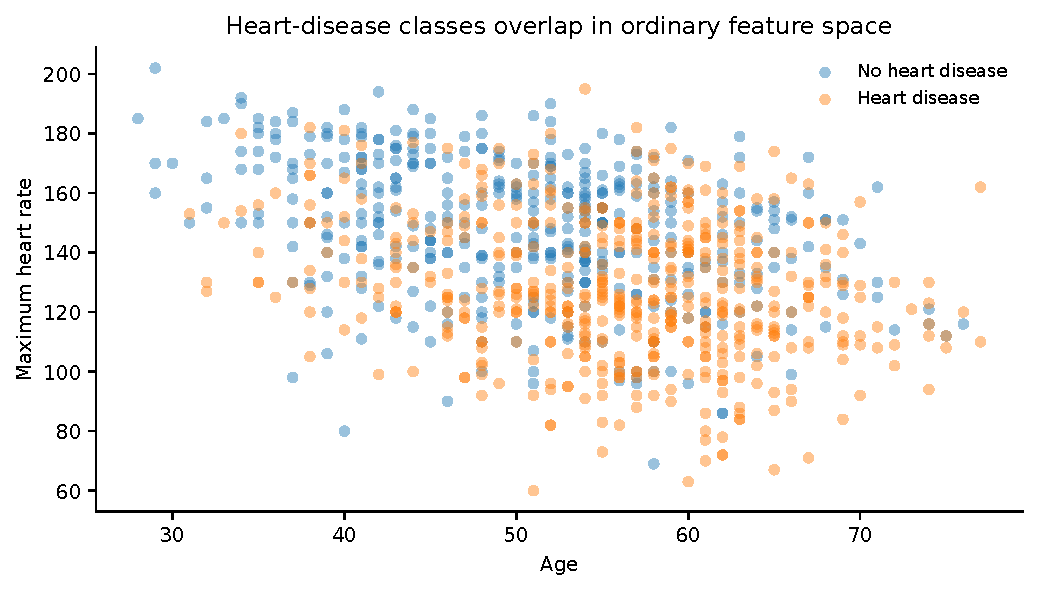
\includegraphics[width=0.80\linewidth]{figures_generated/classification_heart_age_maxhr.pdf}
\end{utpfig}

Heart disease is present in about 55.3\% of the 918 records. Mean maximum heart rate is lower in the labelled heart-disease group (about 128) than in the non-disease group (about 148), but the distributions overlap. Categorical predictors such as chest-pain type and ST slope contribute information that cannot be represented by this two-dimensional picture.

\begin{utpfig}[Breast-cancer measurements show partial separation]{Mean radius and mean texture separate many benign and malignant records, yet overlap remains. The full dataset includes many related measurements, creating both predictive opportunity and redundancy.}{fig:class-breast}
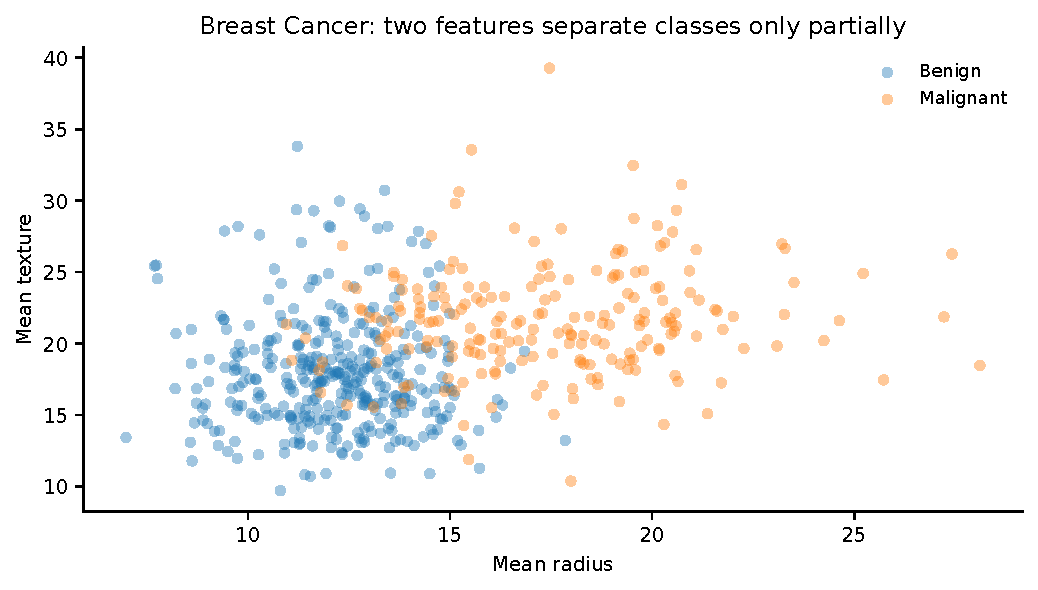
\includegraphics[width=0.80\linewidth]{figures_generated/classification_breast_features.pdf}
\end{utpfig}

In the Breast Cancer file, about 37.3\% of records are malignant. Mean radius averages about 17.46 for malignant records versus 12.15 for benign records. A classifier can exploit such differences, but evaluation must be performed on unseen data and should report error types that match the decision context.

\section{High-dimensional extension: handwritten digits}

The bundled \texttt{optical\_recognition\_handwritten\_digits.zip} contains a training file with 3,823 examples and a test file with 1,797 examples. Each observation contains 64 pixel-intensity features arranged conceptually as an $8\times8$ image plus a digit label from 0 to 9. The values range from 0 to 16 and describe local pixel density rather than a photograph stored as an image file.

\begin{utpfig}[A table row can still represent an image]{The ten panels reconstruct one example of each digit from the 64 numeric feature values. The classifier receives a vector of numbers; the image layout is domain knowledge that helps humans understand what those numbers mean.}{fig:class-digits-examples}
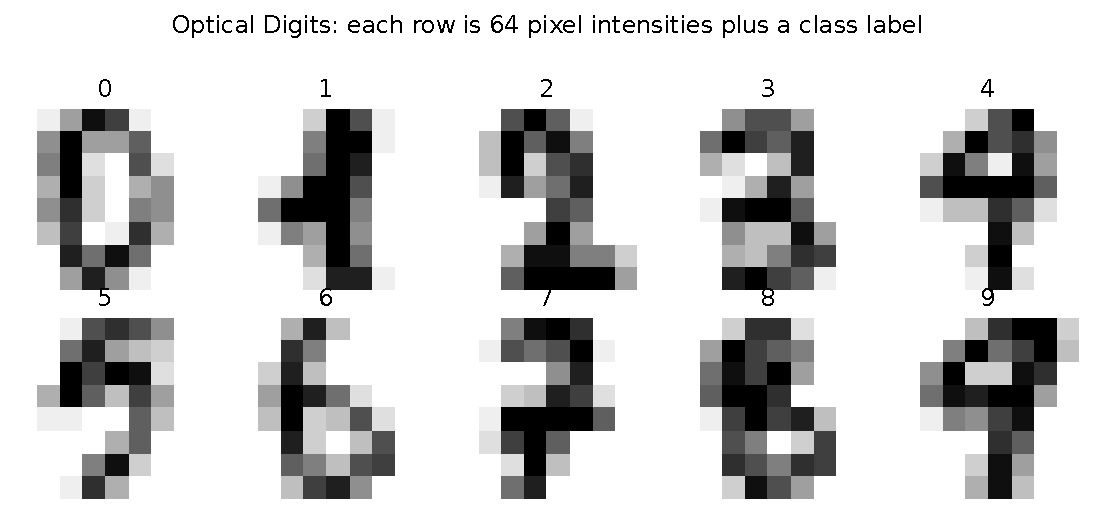
\includegraphics[width=0.86\linewidth]{figures_generated/classification_digits_examples.pdf}
\end{utpfig}

This dataset extends binary classification in three important ways. First, the outcome has ten classes, so evaluation needs a $10\times10$ confusion matrix or per-class metrics rather than one sensitivity/specificity pair. Second, 64 dimensions make direct visualisation impossible. Third, the supplied train/test split reflects different writers, which can be more demanding than randomly mixing records from the same writer across both sets.

\begin{utpfig}[Two dimensions cannot preserve all multiclass structure]{PCA compresses the 64 standardised pixel features into two directions for visual inspection. Some digits form visible regions, but extensive overlap remains; a two-dimensional plot is an interpretation tool, not the classifier itself.}{fig:class-digits-pca}
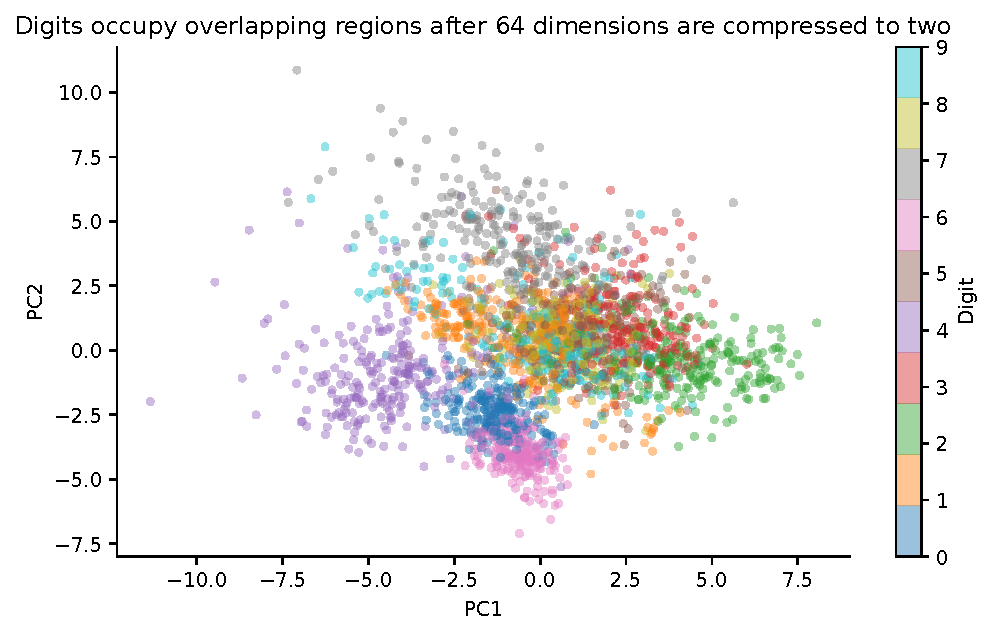
\includegraphics[width=0.80\linewidth]{figures_generated/classification_digits_pca.pdf}
\end{utpfig}

Multiclass performance should be reported at more than one level. Overall accuracy answers ``how often is the label correct?'' while a confusion matrix reveals which digits are confused. Macro-averaged metrics give each digit equal weight; frequency-weighted metrics emphasise common digits. These choices matter whenever class frequencies differ.

\begin{keyidea}
High dimensionality is not only ``many columns.'' It changes distance, visualisation, model complexity, and validation. The digits data provide a bridge from classification to PCA and representation learning while also showing why the data-generating split matters.
\end{keyidea}
